% De la numérisation à l’annotation

\subsection{Chaîne de traitement des sources historiques}
    \subsubsection{Du manuscrit aux diagrammes : chaîne de traitement des sources astronomiques}
	La chaîne de traitement proposée par \eida (fig. \ref{fig:eida_workflow}) propose ainsi une alternance d'étapes automatisées, en bleu sur le schéma, et d'étapes d'analyse par les chercheurs du projet.
	
	\begin{figure}[h]
		\centering
		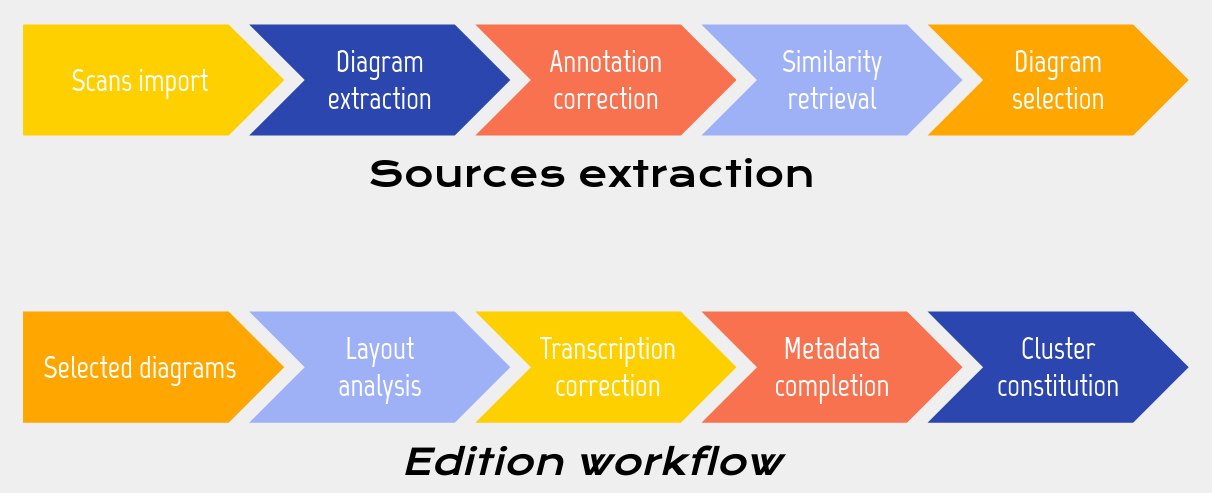
\includegraphics[width=15cm]{images/eida_workflow.png}
		\caption{\textit{Workflow} de traitement des sources du projet \eida}
		\label{fig:eida_workflow}
	\end{figure}

    \subsubsection{Traitements automatiques, traitements manuels}
	qu'est-ce qui peut être automatisé, qu'est-ce qui ne l'est pas, intervention des chercheurs, etc etc
    
    \subsection{Échanges et transformation des données}
        \subsubsection{Sources d'entrée, sources de sortie}
		de l'image au manifeste à l'image, au txt puis sas

        \subsubsection{Traitement des résultats de la détection}
        après avoir obtenu les diagrammes : deux possibilités, plus de traitements automatiques, cf partie 3, ou résultat en lui même
        
        par exemple détection d'objets permet de constituer un corpus qui sera traité manuellement ?

    \subsection{Créer des interfaces pour les étapes manuelles}
        \subsubsection{Correction par les chercheurs : au-delà de l'entraînement}
        expliquer que la correction se fait pas juste pour l'entraînement mais que l'interface permettra plus tard aux chercheurs de sélectionner les diagrammes qui les intéressent

        \subsubsection{Interface d'annotation}
		interface pour les chercheurs, pour la correction : captures d'écran 
		réelles réflexions techniques pour la praticité 
